\documentclass[10pt]{article}
\usepackage[margin=18mm]{geometry}
\usepackage{graphicx,booktabs,hyperref}
\usepackage[strings]{underscore}
\setlength{\parindent}{0pt}\setlength{\parskip}{5pt}
\begin{document}
\section*{Correctness controls and retained refusals}
Cohorts: selftest-20261023-01/02/03, fixture-replay-20261023-01,
aa-original-20261023-01 and query-audit[-d2/-d3]-20261023-01.
These are correctness and replay controls, not independent performance trials.

The final selftest passes for n=5,7, ell=1,2 and all four basis families.
All seven original fixture counts agree independently, including checked
witnesses on all three SAT draws. Original n19/ell4/geometric/rep0 A/A
checks all 12 rows after excluding only diagnostic seconds: every other
field equals the original panel. Independent direct group enumeration checks
every completed extraction in each of the three structural panels, with
zero failures. Partial extractions stay partial.

\begin{center}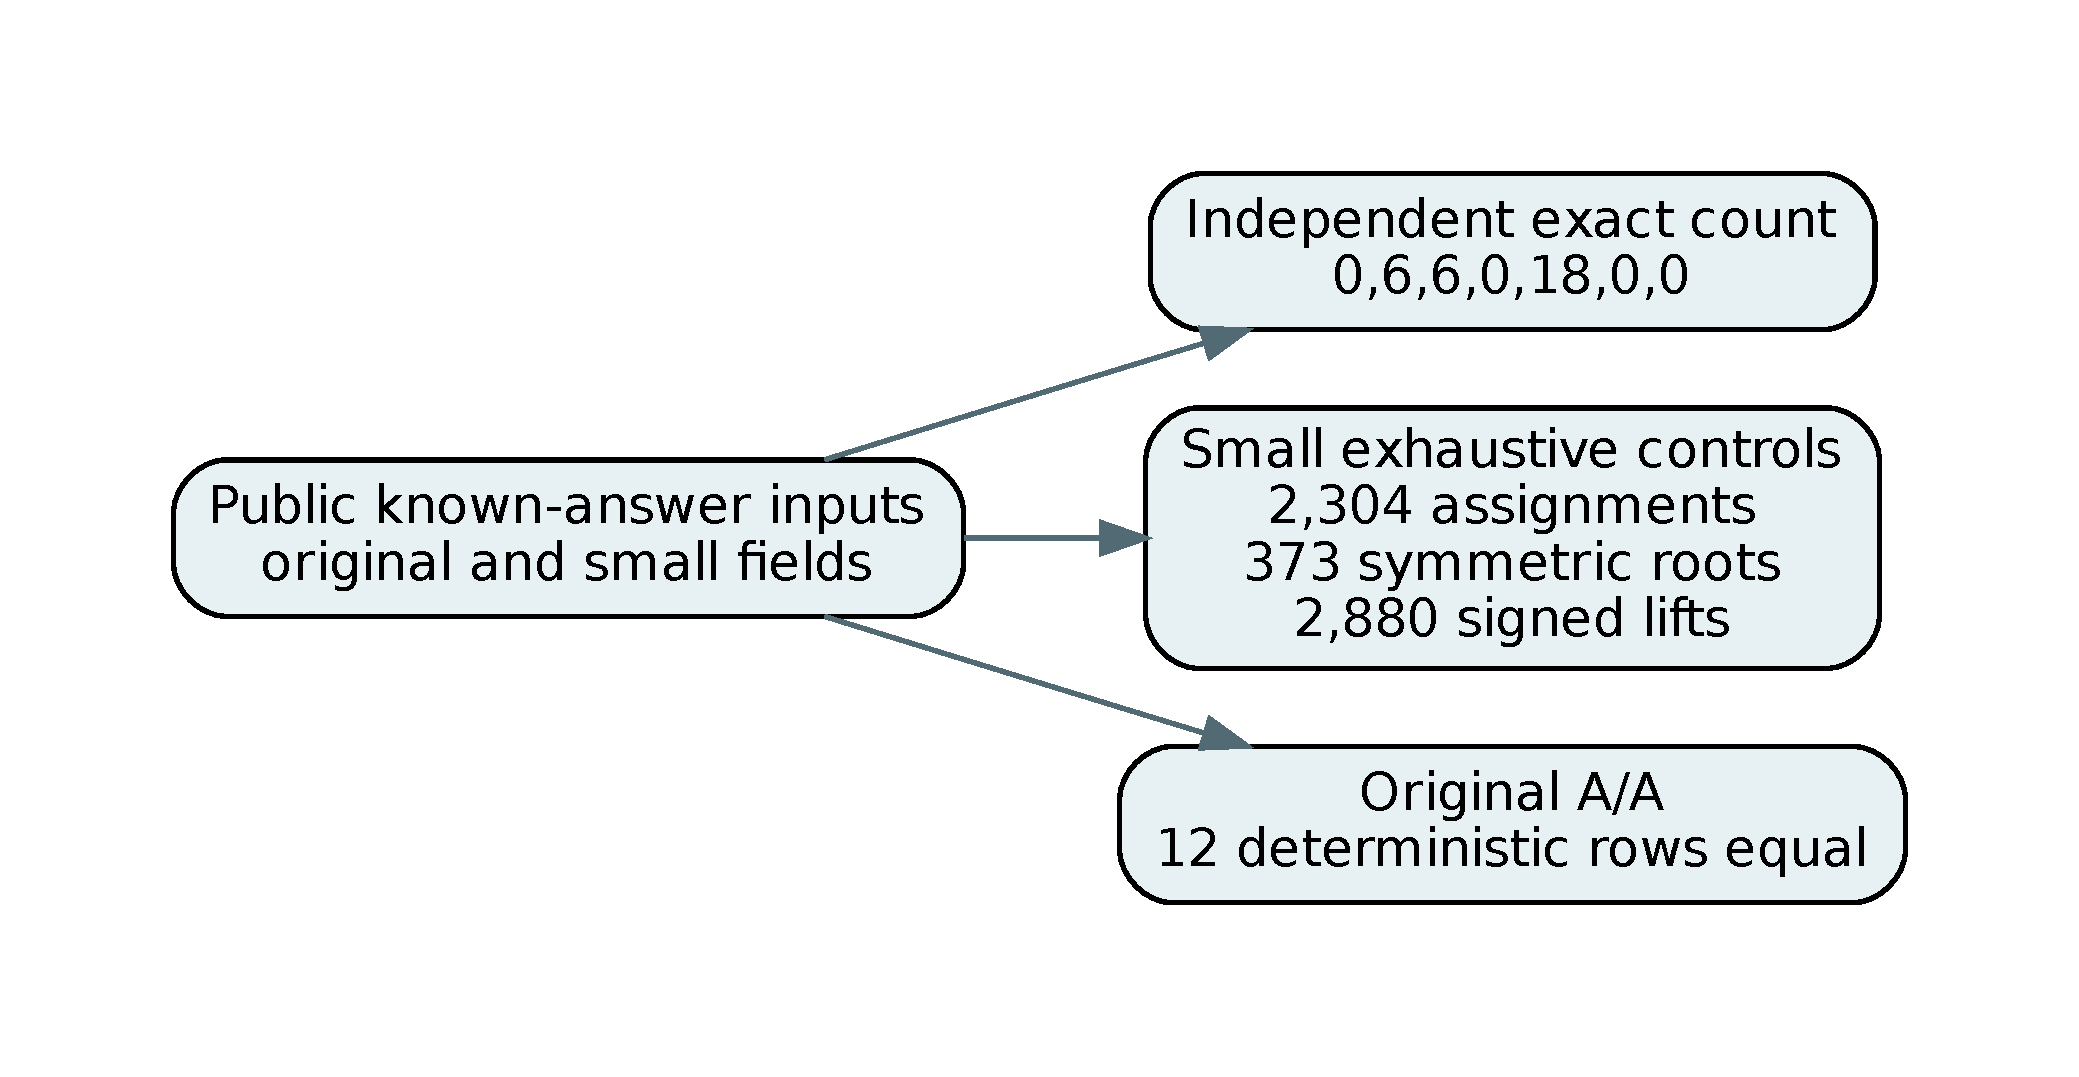
\includegraphics[width=.97\linewidth]{control-paths.pdf}\end{center}

The first selftest attempt exited 127 because GNU time was absent; the first
structural orchestration failed at jq argument parsing before a native
measurement. Their empty output is not a zero-cost result. The final
degree-four structural shell had a separate syntax error after all 96
native commands succeeded, caused by editing its active runner on disk.
Later panels use preserved frozen runner copies. These setup failures and
the raw shell-exit receipt remain in the archive.

Native source: \path{examples/ic_algebraic_followup.rs}; each run pins its
own source/binary hashes, and the later instrument build is d67f6085.
Local limits are 12 GiB and
900 seconds per process on the shared x86-64 host, L0. Timings are diagnostic.
Native report recomputation: \path{examples/ic_campaign_report_data.rs};
values and raw SHA-256 pointers in \path{../../report-data.json}.

\newpage\section*{Guess caps, width refusals and certificate}
Balanced k=0/1/2 attempts ran every branch across the four original UNSAT
draws, 4/8/16 processes respectively. All 28 return column-cap, not a
degree verdict. Eight initial k=3 draw-0 processes returned engine-cap
under the library's default 40,000-column cap; they are unscored. Raising
only the internal cap to the already declared instrument limit permits the
separate complete eight-branch run, whose report is a sibling.

Native ecbench plan at m=16,17,18 returns exit 2, explicitly outside the
supported quartic base-field range 4--15. Coefficients, sentinels, packed
coordinates and scalars need a wider implementation; this is not a
mathematical exclusion. No quartic solve or cost follows from a refusal.

The summand-exchange check, certificate IDC1ha27a77e72057f9cb, independently
normalizes both S3 integer polynomials (six terms, maximum coefficient two),
checks the standard finite-field certificate, and checks the bit permutation
on all 308 equations of the seven original inputs. The two generated JSON
artifacts reproduce byte for byte in a later process. Its formal-proof
pointer is unset. It relates degree verdicts for [7,23,24] and [15,23,24],
not their measured costs or an untested minimum.

Raw records: the \path{runs/} tree in
\path{../../evidence/runs-local-20261023.tar.xz}, including commands,
source revisions, stderr, exit codes, host and memory receipts. The native
inventory lists all 33 run directories and hashes their raw rows. Refusal
sidecars are included separately. The frozen protocol and its amendments
identify the setup and degree-floor deviations.

Certificate source and artifacts: \path{examples/ic_guess_symmetry.rs},
\path{../../proofs/s3-swap.identity.json}, and
\path{../../proofs/guess-swap.receipt.json}.
No comparable timing samples are admitted, so the visual is a control-path
diagram. No fastest-CAS, GPU, asymptotic or security claim follows.

\end{document}
